\chapter{Introduction to Probability}\label{probability_chap}

%% Introduction %%%%%%%%%%%%%%%%%%%%%%%%%%%%%%%%%%%%%%%%%%%%%%%%%%%%%%%%%%%%%%%

Probability plays a key role in the sciences ---''hard'' and social
---including computer science.  Many algorithms rely on randomization.
Investigating their correctness and performance requires probability
theory.  Moreover, computer systems designs, such as memory management,
branch prediction, packet routing, and load balancing are based on
probabilistic assumptions and analyses.  Probability is central as well in
related subjects such as information theory, cryptography, artificial
intelligence, and game theory.  But we'll start with a more down-to-earth
application: getting a prize in a game show.

\iffalse
Beyond these engineering applications, probability gives
insight into everyday issues like such as polling, DNA testing, risk
assessment, investing, and gambling.
\fi


%% Monty Hall %%%%%%%%%%%%%%%%%%%%%%%%%%%%%%%%%%%%%%%%%%%%%%%%%%%%%%%%%%%%%%%%%
\section{Monty Hall}\label{monty_sec}

In the September 9, 1990 issue of \textit{Parade} magazine, the
columnist Marilyn vos Savant responded to this letter:

%  future:
%  Include the other problem that Marilyn addressed in the same issue.

\begin{quotation}
\noindent \textit{Suppose you're on a game show, and you're given the
choice of three doors.  Behind one door is a car, behind the others,
goats.  You pick a door, say number 1, and the host, who knows what's
behind the doors, opens another door, say number 3, which has a goat.
He says to you, "Do you want to pick door number 2?"  Is it to your
advantage to switch your choice of doors?}

\vspace{1ex}

\hspace{3in} Craig. F. Whitaker

\hspace{3in} Columbia, MD
\end{quotation}

The letter describes a situation like one faced by contestants on the
1970's game show \textit{Let's Make a Deal}, hosted by Monty Hall and
Carol Merrill.  Marilyn replied that the contestant should indeed switch.
She explained that if the car was behind either of the two unpicked doors
---which is twice as likely as the the car being behind the picked door
---the contestant wins by switching.  But she soon received a torrent of
letters, many from mathematicians, telling her that she was wrong.  The
problem generated thousands of hours of heated debate.

This incident highlights a fact about probability: the subject uncovers
lots of examples where ordinary intuition leads to completely wrong
conclusions.  So until you've studied probabilities enough to have
refined your intuition, a way to avoid errors is to fall back on a
rigorous, systematic approach such as the Four Step Method.

\subsection{The Four Step Method}

Every probability problem involves some sort of randomized experiment,
process, or game.  And each such problem involves two distinct
challenges:
%
\begin{enumerate}
\item How do we model the situation mathematically?
\item How do we solve the resulting mathematical problem?
\end{enumerate}
%
In this section, we introduce a four step approach to questions of the
form, ``What is the probability that ----- ?''  In this approach, we build
a probabilistic model step-by-step, formalizing the original question in
terms of that model.  Remarkably, the structured thinking that this
approach imposes provides simple solutions to many famously-confusing
problems.  For example, as you'll see, the four step method cuts through
the confusion surrounding the Monty Hall problem like a Ginsu knife.
However, more complex probability questions may spin off challenging
counting, summing, and approximation problems--- which, fortunately,
you've already spent weeks learning how to solve.

\subsection{Clarifying the Problem}

Craig's original letter to Marilyn vos Savant is a bit vague, so we
must make some assumptions in order to have any hope of modeling the
game formally:
%
\begin{enumerate}

\item The car is equally likely to be hidden behind each of the three
doors.

\item The player is equally likely to pick each of the three doors,
regardless of the car's location.

\item After the player picks a door, the host {\em must} open a
different door with a goat behind it and offer the player the choice
of staying with the original door or switching.

\item If the host has a choice of which door to open, then he is
equally likely to select each of them.

\end{enumerate}
%
In making these assumptions, we're reading a lot into Craig Whitaker's
letter.  Other interpretations are at least as defensible, and some
actually lead to different answers.  But let's accept these
assumptions for now and address the question, ``What is the
probability that a player who switches wins the car?''

\subsection{Step 1:  Find the Sample Space}

Our first objective is to identify all the possible outcomes of the
experiment.  A typical experiment involves several randomly-determined
quantities.  For example, the Monty Hall game involves three such
quantities:
%
\begin{enumerate}
\item The door concealing the car.
\item The door initially chosen by the player.
\item The door that the host opens to reveal a goat.
\end{enumerate}
%
Every possible combination of these randomly-determined quantities is
called an \term{outcome}.  The set of all possible outcomes is called
the \term{sample space} for the experiment.

A \term{tree diagram} is a graphical tool that can help us work
through the four step approach when the number of outcomes is not too
large or the problem is nicely structured.  In particular, we can use
a tree diagram to help understand the sample space of an experiment.
The first randomly-determined quantity in our experiment is the door
concealing the prize.  We represent this as a tree with three
branches:
\begin{center}
\mfigure{!}{2.5in}{figures/monty1}
\end{center}
In this diagram, the doors are called $A$, $B$, and $C$ instead of 1, 2,
and 3 because we'll be adding a lot of other numbers to the picture later.

Now, for each possible location of the prize, the player could initially
choose any of the three doors.  We represent this in a second layer added to
the tree.  Then a third layer represents the possibilities of the final step when
the host opens a door to reveal a goat:

\begin{staffnotes}

\begin{center}
\mfigure{!}{3.3in}{monty2}
\end{center}

\end{staffnotes}


\begin{center}
\mfigure{!}{4.0in}{figures/monty3}
\end{center}

Notice that the third layer reflects the fact that the host has either one
choice or two, depending on the position of the car and the door initially
selected by the player.  For example, if the prize is behind door A and
the player picks door B, then the host must open door C.  However, if the
prize is behind door A and the player picks door A, then the host could
open either door B or door C.

Now let's relate this picture to the terms we introduced earlier: the
leaves of the tree represent \textit{outcomes} of the experiment, and
the set of all leaves represents the \textit{sample space}.  Thus, for
this experiment, the sample space consists of 12 outcomes.  For
reference, we've labeled each outcome with a triple of doors
indicating:
%
\[
(\text{door concealing prize}, \ \text{door initially chosen}, \ \text{door opened to reveal a goat})
\]
%
In these terms, the sample space is the set:
%
\[
\set{
\begin{array}{cccccc}
(A, A, B), & (A, A, C), & (A, B, C), & (A, C, B), & (B, A, C), & (B, B, A), \\
(B, B, C), & (B, C, A), & (C, A, B), & (C, B, A), & (C, C, A), & (C, C, B)
\end{array}}
\]
%
The tree diagram has a broader interpretation as well: we can regard the
whole experiment as following a path from the root to a leaf, where the
branch taken at each stage is ``randomly'' determined.  Keep this
interpretation in mind; we'll use it again later.

\subsection{Step 2: Define Events of Interest}

Our objective is to answer questions of the form ``What is the probability
that \dots ?'', where the missing phrase might be ``the player wins by
switching'', ``the player initially picked the door concealing the
prize'', or ``the prize is behind door C'', for example.  Each of these
phrases characterizes a set of outcomes: the outcomes
specified by ``the prize is behind door $C$'' is:
%
\[
\set{(C, A, B), (C, B, A), (C, C, A), (C, C, B)}
\]
%
A set of outcomes is called an \term{event}.  So the event that the player
initially picked the door concealing the prize is the set:
%
\[
\set{(A, A, B), (A, A, C), (B, B, A), (B, B, C), (C, C, A), (C, C, B)}
\]
%
And what we're really after, the event that the player wins by
switching, is the set of outcomes:
%
\[
\set{(A, B, C), (A, C, B), (B, A, C), (B, C, A), (C, A, B), (C, B, A)}
\]
%
%These are the outcomes labelled with ``X'' in the diagram above.
%\iffalse
Let's annotate our tree diagram to indicate the outcomes in this
event.
%
\begin{center}
\mfigure{!}{3.5in}{figures/monty4}
\end{center}
%\fi
Notice that exactly half of the outcomes are marked, meaning that the
player wins by switching in half of all outcomes.  You might be
tempted to conclude that a player who switches wins with probability
$1/2$.  \textit{This is wrong.}  The reason is that these
outcomes are not all equally likely, as we'll see shortly.

\subsection{Step 3: Determine Outcome Probabilities}

So far we've enumerated all the possible outcomes of the experiment.  Now
we must start assessing the likelihood of those outcomes.  In particular,
the goal of this step is to assign each outcome a probability, indicating
the fraction of the time this outcome is expected to occur.  The sum of
all outcome probabilities must be one, reflecting the fact that there
always is an outcome.

Ultimately, outcome probabilities are determined by the phenomenon
we're modeling and thus are not quantities that we can derive
mathematically.  However, mathematics can help us compute the
probability of every outcome \textit{based on fewer and more
elementary modeling decisions.}  In particular, we'll break the task
of determining outcome probabilities into two stages.

\subsubsection{Step 3a: Assign Edge Probabilities}

First, we record a probability on each \textit{edge} of the tree
diagram.  These edge-probabilities are determined by the assumptions
we made at the outset: that the prize is equally likely to be behind
each door, that the player is equally likely to pick each door, and
that the host is equally likely to reveal each goat, if he has a
choice.  Notice that when the host has no choice regarding which door
to open, the single branch is assigned probability 1.
%
\begin{center}
\mfigure{!}{3.5in}{figures/monty5}
\end{center}

\subsubsection{Step 3b: Compute Outcome Probabilities}

Our next job is to convert edge probabilities into outcome
probabilities.  This is a purely mechanical process: \textit{the
probability of an outcome is equal to the product of the
edge-probabilities on the path from the root to that outcome}.  For
example, the probability of the topmost outcome, $(A, A, B)$ is
\[
\frac{1}{3} \cdot \frac{1}{3} \cdot \frac{1}{2} = \frac{1}{18}.
\]

There's an easy, intuitive justification for this rule.  As the steps in
an experiment progress randomly along a path from the root of the tree to
a leaf, the probabilities on the edges indicate how likely the walk is to
proceed along each branch.  For example, a path starting at the root in
our example is equally likely to go down each of the three top-level
branches.

Now, how likely is such a walk to arrive at the topmost outcome, $(A,
A, B)$?  Well, there is a 1-in-3 chance that a walk would follow the
$A$-branch at the top level, a 1-in-3 chance it would continue along
the $A$-branch at the second level, and 1-in-2 chance it would follow
the $B$-branch at the third level.  Thus, it seems that about 1 walk
in 18 should arrive at the $(A, A, B)$ leaf, which is precisely the
probability we assign it.

Anyway, let's record all the outcome probabilities in our tree
diagram.
%
\begin{center}

\mfigure{!}{3.5in}{figures/monty6}
\end{center}

Specifying the probability of each outcome amounts to defining a
function that maps each outcome to a probability.  This function is
usually called \textbf{Pr}.  In these terms, we've just determined
that:
%
\begin{align*}
\pr{(A, A, B)} & = \frac{1}{18} \\
\pr{(A, A, C)} & = \frac{1}{18} \\
\pr{(A, B, C)} & = \frac{1}{9} \\
               & \text{etc.}
\end{align*}

\subsection{Step 4: Compute Event Probabilities}

We now have a probability for each \textit{outcome}, but we want to
determine the probability of an \textit{event} which will be the sum of
the probabilities of the outcomes in it.  The probability of an event,
$E$, is written $\pr{E}$.  For example, the probability of the event that
the player wins by switching is:
%
\begin{align*}
\pr{\text{switching wins}}
    & = \pr{(A, B, C)} + \pr{(A, C, B)} + \pr{(B, A, C)} + \\
    & \qquad \pr{(B, C, A)} + \pr{(C, A, B)} + \pr{(C, B, A)} \\
    & = \frac{1}{9} + \frac{1}{9} + \frac{1}{9} + 
        \frac{1}{9} + \frac{1}{9} + \frac{1}{9} \\
    & = \frac{2}{3}
\end{align*}
%
It seems Marilyn's answer is correct; a player who switches doors wins
the car with probability $2/3$!  In contrast, a player who stays with
his or her original door wins with probability $1/3$, since staying
wins if and only if switching loses.

We're done with the problem!  We didn't need any appeals to intuition
or ingenious analogies.  In fact, no mathematics more difficult than
adding and multiplying fractions was required.  The only hard part was
resisting the temptation to leap to an ``intuitively obvious'' answer.

\subsection{An Alternative Interpretation of the Monty Hall Problem}

Was Marilyn really right?  Our analysis suggests she was.  But a more
accurate conclusion is that her answer is correct \textit{provided we
accept her interpretation of the question}.  There is an equally
plausible interpretation in which Marilyn's answer is wrong.  Notice
that Craig Whitaker's original letter does not say that the host is
\textit{required} to reveal a goat and offer the player the option to
switch, merely that he \textit{did} these things.  In fact, on the
\textit{Let's Make a Deal} show, Monty Hall sometimes simply opened
the door that the contestant picked initially.  Therefore, if he
wanted to, Monty could give the option of switching only to
contestants who picked the correct door initially.  In this case,
switching never works!

%% Monty Hall Problems %%%%%%%%%%%%%%%%%%%%%%%%%%%%%%%%%%%%%%%%%%%%%%%%%%%%%%%%

\begin{problems}
\classproblems
\pinput{CP_a_baseball_series}
\pinput{CP_coin_flips}
\pinput{CP_the_four_door_deal}
\pinput{CP_simulating_fair_coin}

\homeworkproblems
\pinput{PS_black_and_red_cards}

\end{problems}

%% Set Theory and Probability %%%%%%%%%%%%%%%%%%%%%%%%%%%%%%%%%%%%%%%%%%%%%%%%%
\section{Set Theory and Probability}

Let's abstract what we've just done in this Monty Hall example into a
general mathematical definition of probability.  In the Monty Hall
example, there were only finitely many possible outcomes.  Other examples
in this course will have a countably infinite number of outcomes.

General probability theory deals with uncountable sets like the set of
real numbers, but we won't need these, and sticking to countable sets lets
us define the probability of events using sums instead of integrals.  It
also lets us avoid some distracting technical problems in set theory like
the Banach-Tarski ``paradox'' mentioned in Chapter~\ref{setsreallywork}.

\subsection{Probability Spaces}

\begin{definition}\label{LN12:sampsp}
  A countable \term{sample space}, $\sspace$, is a nonempty countable set.
  An element $w \in \sspace$ is called an \term{outcome}.  A subset of
  $\sspace$ is called an \term{event}.
\end{definition}

\begin{definition}\label{LN12:probsp}
 A \term{probability function} on a sample space, $\sspace$, is a total
 function $\pr{}: \sspace\to \reals$ such that
\begin{itemize}
\item $\pr{w} \geq 0$ for all $w \in \sspace$, and
\item $\sum_{w \in \sspace} \pr{w} = 1$.
\end{itemize}
The sample space together with a probability function is called a
\hyperdef{prob}{space}{\term{probability space}}.

For any event, $E \subseteq \sspace$, the \index{probability of an event}
\emph{probability of $E$} is defined to be the sum of the probabilities of
the outcomes in $E$:
\[
\pr{E} \eqdef \sum_{w \in E} \pr{w}.
\]
\end{definition}

An immediate consequence of the definition of event probability is that
for \emph{disjoint} events, $E,F$,
\[
\pr{E \union F} = \pr{E} + \pr{F}.
\]
This generalizes to a countable number of events.  Namely, a collection of
sets is \term{pairwise disjoint} when no element is in more than one of
them ---formally, $A \intersect B = \emptyset$ for all sets $A \neq B$ in
the collection.

\begin{rul*} [\idx{Sum Rule}] 
  If $\set{E_0,E_1,\dots}$ is collection of pairwise disjoint events, then
\[
\pr{\lgunion_{n\in\naturals}E_n} = \sum_{n\in\naturals} \pr{E_n}.
\]
\end{rul*}

The Sum Rule\footnote{If you think like a mathematician, you should be
   wondering if the infinite sum is really necessary.  Namely, suppose we
   had only used finite sums in Definition~\ref{LN12:probsp} instead of sums
   over all natural numbers.  Would this imply the result for infinite
   sums?  It's hard to find counterexamples, but there are some: it is
   possible to find a pathological ``probability'' measure on a sample
   space satisfying the Sum Rule for finite unions, in which the outcomes
   $w_0,w_1,\dots$ each have probability zero, and the probability
   assigned to any event is either zero or one!  So the infinite Sum Rule
   fails dramatically, since the whole space is of measure one, but it is
   a union of the outcomes of measure zero.

   The construction of such weird examples is beyond the scope of this
   text.  You can learn more about this by taking a course in Set
   Theory and Logic that covers the topic of ``ultrafilters.''}  lets
us analyze a complicated event by breaking it down into simpler cases.
For example, if the probability that a randomly chosen MIT student is
native to the United States is 60\%, to Canada is 5\%, and to Mexico
is 5\%, then the probability that a random MIT student is native to
North America is 70\%.

Another consequence of the Sum Rule is that $\pr{A} + \pr{\bar{A}} = 1$,
which follows because $\pr{\sspace}=1$ and $\sspace$ is the union of the
disjoint sets $A$ and $\bar{A}$.  This equation often comes up in the form
\begin{rul*} [\idx{Complement Rule}]
\[
\pr{\bar{A}}  =  1 - \pr{A}.
\]
\end{rul*}
Sometimes the easiest way to compute the probability of an event is to compute
the probability of its complement and then apply this formula.

Some further basic facts about probability parallel facts about
cardinalities of finite sets.  In particular:
\begin{align}
\pr{B-A}        & =  \pr{B} - \pr{A \intersect B},\tag{Difference Rule}\\
\pr{A \union B} & =  \pr{A} + \pr{B} - \pr{A \intersect B},
                  \tag{Inclusion-Exclusion}\\
\pr{A \union B} & \le  \pr{A} + \pr{B}. \tag{Boole's Inequality}
\end{align}
The \idx{Difference Rule} follows from the Sum Rule because $B$ is the
union of the disjoint sets $B-A$ and $A \intersect B$.
\index{inclusion-exclusion for probabilities} Inclusion-Exclusion then
follows from the Sum and Difference Rules, because $A \union B$ is the
union of the disjoint sets $A$ and $B-A$.  \idx{Boole's inequality} is an
immediate consequence of Inclusion-Exclusion since probabilities are
nonnegative.

The two event Inclusion-Exclusion equation above generalizes to $n$ events
in the same way as the corresponding Inclusion-Exclusion rule for $n$
sets.  Boole's inequality also generalizes to
\begin{equation}
\pr{E_1 \cup \cdots \cup E_n} \leq \pr{E_1} + \cdots + \pr{E_n}.\tag{Union Bound}
\end{equation}
This simple \idx{Union Bound} is actually useful in many calculations.
For example, suppose that $E_i$ is the event that the $i$-th critical
component in a spacecraft fails.  Then $E_1 \cup \cdots \cup E_n$ is the
event that \emph{some} critical component fails.  The Union Bound can give
an adequate upper bound on this vital probability.

Similarly, the Difference Rule implies that
\hyperdef{ln10}{monotonicity}{
\begin{equation}\label{LN12:subsetbound}
\text{If } A \subseteq B, \text{ then } \pr{A} \le \pr{B}.\tag{Monotonicity}
\end{equation}}


\subsection{An Infinite Sample Space}

Suppose two players take turns flipping a fair coin.  Whoever flips
heads first is declared the winner.  What is the probability that the
first player wins?  A tree diagram for this problem is shown below:

\mfigure{!}{2in}{figures/infinite-tree1}

The event that the first player wins contains an infinite number of
outcomes, but we can still sum their probabilities:
\begin{align*}
\pr{\text{first player wins}}
    & = \frac{1}{2} + \frac{1}{8} + \frac{1}{32} + \frac{1}{128} + \cdots \\
    & = \frac{1}{2} \sum_{n=0}^\infty \paren{\frac{1}{4}}^n \\
    & = \frac{1}{2}\paren{\frac{1}{1-1/4}} = \frac{2}{3}.
\end{align*}

Similarly, we can compute the probability that the second player wins:
\begin{align*}
\pr{\text{second player wins}}
    & = \frac{1}{4} + \frac{1}{16} + \frac{1}{64} + \frac{1}{256}
                      + \cdots \\
    & = \frac{1}{3}.
\end{align*}

To be formal about this, sample space is the infinite set
\[
\sspace \eqdef \set{\mathtt{T}^n\mathtt{H} \suchthat n \in \naturals}
\]
where $\mathtt{T}^n$ stands for a length $n$ string of $\mathtt{T}$'s.
The probability function is
\[
\pr{\mathtt{T}^n\mathtt{H}} \eqdef \frac{1}{2^{n+1}}.
\]
Since this function is obviously nonnegative, To verify that this is a
probability space, we just have to check that all the probabilities
sum to 1.  But this follows directly from the formula for the sum of a
geometric series:
\[
\sum_{\mathtt{T}^n\mathtt{H} \in \sspace} \pr{\mathtt{T}^n\mathtt{H}} =
\sum_{n \in \naturals} \frac{1}{2^{n+1}} = \frac{1}{2}\sum_{n \in
  \naturals} \frac{1}{2^n} = 1.
\]

Notice that this model does not have an outcome corresponding to the
possibility that both players keep flipping tails forever ---in the
diagram, flipping forever corresponds to following the infinite path
in the tree without ever reaching a leaf/outcome.  If leaving this
possibility out of the model bothers you, you're welcome to fix it by
adding another outcome, $w_{\text{forever}}$, to indicate that that's
what happened.  Of course since the probabililities of the other
outcomes already sum to 1, you have to define the probability of
$w_{\text{forever}}$ to be 0.  Now outcomes with probability zero will
have no impact on our calculations, so there's no harm in adding it in
if it makes you happier.  On the other hand, there's also no harm in
simply leaving it out as we did, since it has no impact.

The mathematical machinery we've developed is adequate to model and
analyze many interesting probability problems with infinite sample
spaces.  However, some intricate infinite processes require
uncountable sample spaces along with more powerful (and more complex)
measure-theoretic notions of probability.  For example, if we generate
an infinite sequence of random bits $b_1, b_2, b_3, \ldots$, then what
is the probability that
\[
\frac{b_1}{2^1} + \frac{b_2}{2^2} + \frac{b_3}{2^3} + \cdots
\]
is a rational number?  Fortunately, we won't have any need to worry about
such things.


%% Set Theory and Probability Problems %%%%%%%%%%%%%%%%%%%%%%%%%%%%%%%%%%%%%%%%
\begin{problems}
\classproblems
\pinput{CP_system_component_failure}
\pinput{CP_proving_probability_rules}
\pinput{PS_conditional_space}
\end{problems}

%% Conditional Probability %%%%%%%%%%%%%%%%%%%%%%%%%%%%%%%%%%%%%%%%%%%%%%%%%%%%
\hyperdef{cond}{prob}{\section{Conditional Probability}}

Suppose that we pick a random person in the world.  Everyone has an
equal chance of being selected.  Let $A$ be the event that the person
is an MIT student, and let $B$ be the event that the person lives in
Cambridge.  What are the probabilities of these events?  Intuitively,
we're picking a random point in the big ellipse shown below and asking
how likely that point is to fall into region $A$ or $B$:
%
\begin{center}
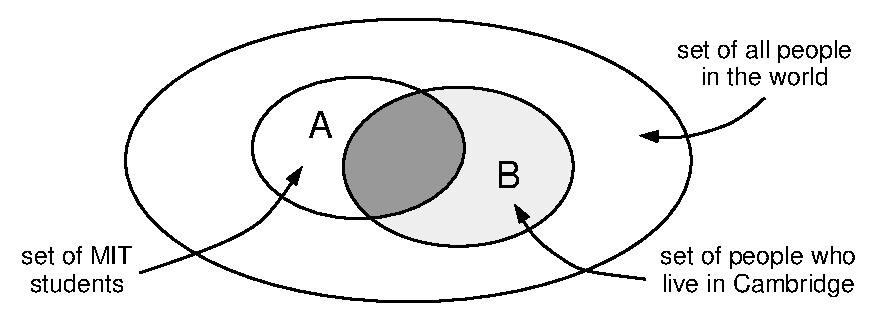
\includegraphics[height=2in]{figures/cambridge-conditional}
\end{center}
%
The vast majority of people in the world neither live in Cambridge nor
are MIT students, so events $A$ and $B$ both have low probability.
But what is the probability that a person is an MIT student,
\textit{given} that the person lives in Cambridge?  This should be
much greater--- but what is it exactly?

What we're asking for is called a \term{conditional probability}; that
is, the probability that one event happens, given that some other
event definitely happens.  Questions about conditional probabilities
come up all the time:
%
\begin{itemize}
\item What is the probability that it will rain this afternoon, given
that it is cloudy this morning?
\item What is the probability that two rolled dice sum to 10, given
that both are odd?
\item What is the probability that I'll get four-of-a-kind in Texas No
Limit Hold 'Em Poker, given that I'm initially dealt two queens?
\end{itemize}

There is a special notation for conditional probabilities.  In
general, $\prcond{A}{B}$ denotes the probability of event $A$, given
that event $B$ happens.  So, in our example, $\prcond{A}{B}$ is the
probability that a random person is an MIT student, given that he or
she is a Cambridge resident.

How do we compute $\prcond{A}{B}$?  Since we are \textit{given} that
the person lives in Cambridge, we can forget about everyone in the
world who does not.  Thus, all outcomes outside event $B$ are
irrelevant.  So, intuitively, $\prcond{A}{B}$ should be the fraction
of Cambridge residents that are also MIT students; that is, the answer
should be the probability that the person is in set $A \intersect B$ (darkly
shaded) divided by the probability that the person is in set $B$
(lightly shaded).  This motivates the definition of conditional
probability:
\begin{definition}\label{LN12:prcond}
\[
\prcond{A}{B} \eqdef \frac{\pr{A \intersect B}}{\pr{B}}
\]
\end{definition}
If $\pr{B} = 0$, then the conditional probability $\prcond{A}{B}$ is
undefined.

Pure probability is often counterintuitive, but conditional probability is
worse!  Conditioning can subtly alter probabilities and produce unexpected
results in randomized algorithms and computer systems as well as in
betting games.  Yet, the mathematical definition of conditional
probability given above is very simple and should give you no trouble---
provided you rely on formal reasoning and not intuition.

\subsection{The ``Halting Problem''}

The \emph{Halting Problem} was the first example of a property that could
not be tested by any program.  It was introduced by Alan Turing in his
seminal 1936 paper.  The problem is to determine whether a Turing machine
halts on a given \dots yadda yadda yadda \dots what's much \emph{more
  important}, it was the name of the MIT EECS department's famed C-league
hockey team.

In a best-of-three tournament, the Halting Problem wins the first game
with probability $1/2$.  In subsequent games, their
probability of winning is determined by the outcome of the previous
game.  If the Halting Problem won the previous game, then they are
invigorated by victory and win the current game with probability
$2/3$.  If they lost the previous game, then they are
demoralized by defeat and win the current game with probablity only
$1/3$.  What is the probability that the Halting Problem wins
the tournament, given that they win the first game?


This is a question about a conditional probability.  Let $A$ be the
event that the Halting Problem wins the tournament, and let $B$ be the
event that they win the first game.  Our goal is then to determine the
conditional probability $\prcond{A}{B}$.

We can tackle conditional probability questions just like ordinary
probability problems: using a tree diagram and the four step method.
A complete tree diagram is shown below, followed by an explanation of
its construction and use.
%
\begin{center}
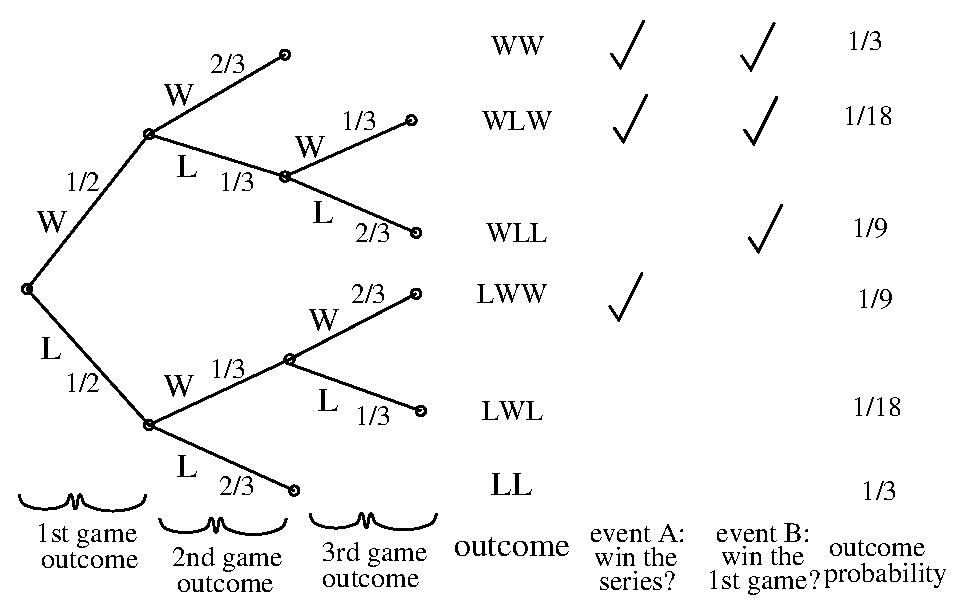
\includegraphics[height=3in]{figures/hockey} % redo this
\end{center}

\subsubsection*{Step 1:  Find the Sample Space}

Each internal vertex in the tree diagram has two children, one
corresponding to a win for the Halting Problem (labeled $W$) and one
corresponding to a loss (labeled $L$).  The complete sample space is:
%
\[
\sspace = \set{ WW,\ WLW,\ WLL,\ LWW,\ LWL,\ LL }
\]

\subsubsection*{Step 2:  Define Events of Interest}

The event that the Halting Problem wins the whole tournament is:
%
\[
T = \set{WW,\ WLW,\ LWW} \\
\]
%
And the event that the Halting Problem wins the first game is:
%
\[
F = \set{WW, WLW, WLL }
\]
%
The outcomes in these events are indicated with checkmarks in the tree
diagram.

\subsubsection*{Step 3:  Determine Outcome Probabilities}

Next, we must assign a probability to each outcome.  We begin by
labeling edges as specified in the problem statement.  Specifically,
The Halting Problem has a $1/2$ chance of winning the first game, so
the two edges leaving the root are each assigned probability $1/2$.
Other edges are labeled $1/3$ or $2/3$ based on the outcome of the
preceding game.  We then find the probability of each outcome by
multiplying all probabilities along the corresponding root-to-leaf
path.  For example, the probability of outcome $WLL$ is:
%
\[
\frac{1}{2} \cdot \frac{1}{3} \cdot \frac{2}{3} = \frac{1}{9}
\]

\subsubsection*{Step 4: Compute Event Probabilities}

We can now compute the probability that The Halting Problem wins the
tournament, given that they win the first game:
%
\begin{align*}
\prcond{A}{B}
    & = \frac{\pr{A \intersect B}}{\pr{B}} \\
    & = \frac{\pr{\set{WW, WLW}}}{\pr{\set{WW, WLW, WLL}}} \\
    & = \frac{1/3 + 1/18}{1/3 + 1/18 + 1/9} \\
    & = \frac{7}{9}
\end{align*}
%
We're done!  If the Halting Problem wins the first game, then they win
the whole tournament with probability $7 / 9$.  


\subsection{Why Tree Diagrams Work}\label{product_rule_subsec}

We've now settled into a routine of solving probability problems using
tree diagrams.  But we've left a big question unaddressed: what is the
mathematical justification behind those funny little pictures?  Why do
they work?

The answer involves conditional probabilities.  In fact, the
probabilities that we've been recording on the edges of tree diagrams
\textit{are} conditional probabilities.  For example, consider the
uppermost path in the tree diagram for the Halting Problem, which
corresponds to the outcome $WW$.  The first edge is labeled $1/2$,
which is the probability that the Halting Problem wins the first game.
The second edge is labeled $2 / 3$, which is the probability that the
Halting Problem wins the second game, \textit{given} that they won the
first--- that's a conditional probability!  More generally, on each
edge of a tree diagram, we record the probability that the experiment
proceeds along that path, given that it reaches the parent vertex.

So we've been using conditional probabilities all along.  But why can
we multiply edge probabilities to get outcome probabilities?  For
example, we concluded that:
%
\begin{align*}
\pr{WW} & = \frac{1}{2} \cdot \frac{2}{3} \\
	& = \frac{1}{3}
\end{align*}
%
Why is this correct?

The answer goes back to Definition~\ref{LN12:prcond} of conditional probability
which could be written in a form called the \term{Product Rule} for
probabilities:
%
\begin{rul*}[Product Rule for 2 Events]
If $\pr{E_1} \neq 0$, then:
%
\[
\pr{E_1 \intersect E_2} = \pr{E_1} \cdot \prcond{E_2}{E_1}
\]
\end{rul*}
%
Multiplying edge probabilities in a tree diagram amounts to evaluating
the right side of this equation.  For example:
%
\begin{align*}
\lefteqn{\pr{\text{win first game} \intersect \text{win second game}}}
		\hspace{0.5in} \\
	& = \pr{\text{win first game}} \cdot
            \prcond{\text{win second game}}{\text{win first game}} \\
	& = \frac{1}{2} \cdot \frac{2}{3}
\end{align*}
%
So the Product Rule is the formal justification for multiplying edge
probabilities to get outcome probabilities!  Of course to justify
multiplying edge probabilities along longer paths, we need a Product Rule
for $n$ events.  The pattern of the $n$ event rule should be apparent from
\begin{rul*}[Product Rule for 3 Events]
\[
\pr{E_1 \intersect E_2 \intersect E_3}
   = \pr{E_1} \cdot \prcond{E_2}{E_1} \cdot \prcond{E_3}{E_2 \intersect E_1}
\]
providing $\pr{E_1 \intersect E_2} \neq 0$.
\end{rul*}
This rule follows from the definition of conditional probability and the
trivial identity
\[
\pr{E_1 \intersect E_2 \intersect E_3} =
\pr{E_1}\cdot \frac{\pr{E_2 \intersect E_1}}{\pr{E_1}} \cdot
      \frac{\pr{E_3 \intersect E_2 \intersect E_1}}{\pr{E_2 \intersect E_1}}
\]


\subsection{The Law of Total Probability}

Breaking a probability calculation into cases simplifies many problems.
The idea is to calculate the probability of an event $A$ by splitting into
two cases based on whether or not another event $E$ occurs.  That is,
calculate the probability of $A \intersect E$ and $A \intersect \bar{E}$.
By the Sum Rule, the sum of these probabilities equals $\pr{A}$.
Expressing the intersection probabilities as conditional probabilities yields
\begin{rul*}[Total Probability]
\[
\pr{A} = \prcond{A}{E} \cdot \pr{E} +
         \prcond{A}{\bar{E}} \cdot \pr{\bar{E}}.
\]
\end{rul*}

For example, suppose we conduct the following experiment.  First, we flip a
coin.  If heads comes up, then we roll one die and take the result.  If
tails comes up, then we roll two dice and take the sum of the two results.
What is the probability that this process yields a 2?  Let $E$ be the
event that the coin comes up heads, and let $A$ be the event that we get a
2 overall.  Assuming that the coin is fair, $\pr{E} = \pr{\bar{E}} = 1/2$.
There are now two cases. If we flip heads, then we roll a 2 on a single
die with probabilty $\prcond{A}{E} = 1/6$.  On the other hand, if we flip
tails, then we get a sum of 2 on two dice with probability
$\prcond{A}{\bar{E}} = 1/36$.  Therefore, the probability that the whole
process yields a 2 is
\[
\pr{A} = \frac{1}{2} \cdot \frac{1}{6} + \frac{1}{2} \cdot \frac{1}{36} =
  \frac{7}{72}.
\]

There is also a form of the rule to handle more than two cases.
\begin{rul*}[Multicase Total Probability]
If $E_1, \dots, E_n$ are pairwise disjoint events whose
union is the whole sample space, then:
\[
\pr{A} = \sum_{i=1}^{n} \prcond{A}{E_i} \cdot \pr{E_i}.
\]

\end{rul*}


\begin{staffnotes}

\subsection{A Coin Problem}
Someone hands you either a fair coin or a trick coin with heads on both
sides.  You flip the coin 100 times and see heads every time.  What can
you say about the probability that you flipped the fair coin?
Remarkably--- nothing!

In order to make sense out of this outrageous claim, let's formalize
the problem.  The sample space is worked out in the tree diagram
below.  We do not know the probability that you were handed the fair
coin initially--- you were just given one coin or the other--- so
let's call that $p$.
%
\begin{center}
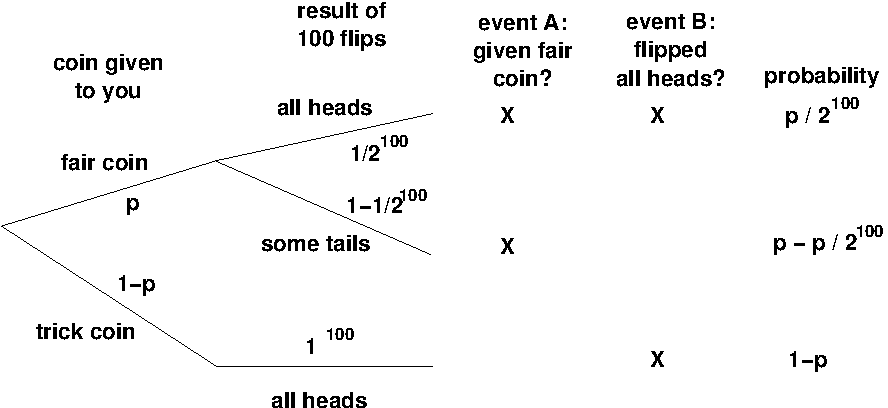
\includegraphics{figures/trick-coin}
\end{center}
%
Let $A$ be the event that you were handed the fair coin, and let $B$
be the event that you flipped 100 heads.  Now, we're looking for
$\prcond{A}{B}$, the probability that you were handed the fair coin,
given that you flipped 100 heads.  The outcome probabilities are
worked out in the tree diagram.  Plugging the results into the
definition of conditional probability gives:
%
\begin{align*}
\prcond{A}{B}	& = \frac{\pr{A \intersect B}}{\pr{B}} \\
		& = \frac{p / 2^{100}}{1 - p + p / 2^{100}} \\
		& = \frac{p}{2^{100} (1 - p) + p}
\end{align*}
%
This expression is very small for moderate values of $p$ because of
the $2^{100}$ term in the denominator.  For example, if $p = 1/2$,
then the probability that you were given the fair coin is essentially
zero.

But we \textit{do not know} the probability $p$ that you were given
the fair coin.  And perhaps the value of $p$ is \textit{not} moderate;
in fact, maybe $p = 1 - 2^{-100}$.  Then there is nearly an even
chance that you have the fair coin, given that you flipped 100 heads.
In fact, maybe you were handed the fair coin with probability $p = 1$.
Then the probability that you were given the fair coin is, well, 1!

A similar problem arises in polling before an election.  A pollster
picks a random American and asks his or her party affiliation.  If
this process is repeated many times, what can be said about the
population as a whole?  To clarify the analogy, suppose that the
country contains only two people.  There is either one Republican and
one Democrat (like the fair coin), or there are two Republicans (like
the trick coin).  The pollster picks a random citizen 100 times, which
is analogous to flipping the coin 100 times.  Suppose that he picks a
Republican every single time.  However, even given this
polling data, the probability that there is one citizen in each party
could still be anywhere between 0 and 1!

What the pollster \textit{can} say is that either:
%
\begin{enumerate}
\item Something earth-shatteringly unlikely happened during the poll.
\item There are two Republicans.
\end{enumerate}
%
This is as far as probability theory can take us; from here, you must
draw your own conclusions.  Based on life experience, many people
would consider the second possibility more plausible.  However, if you
are just \textit{convinced} that the country isn't entirely Republican
(say, because you're a citizen and a Democrat), then you might believe
that the first possibility is actually more likely.

\end{staffnotes}


\subsection{Medical Testing}\label{med_test-subsection}

There is an unpleasant condition called \emph{BO} suffered by 10\% of the
population.  There are no prior symptoms; victims just suddenly start to
stink.  Fortunately, there is a test for latent \emph{BO} before things
start to smell.  The test is not perfect, however:
\begin{itemize}

\item If you have the condition, there is a 10\% chance
that the test will say you do not.  (These are called ``false
negatives''.)

\item If you do not have the condition, there is a 30\% chance that the test
will say you do.  (These are ``false positives''.)

\end{itemize}

Suppose a random person is tested for latent \emph{BO}.  If the test is
positive, then what is the probability that the person has the condition?

\subsubsection*{Step 1: Find the Sample Space}

The sample space is found with the tree diagram below.
%
\begin{center}
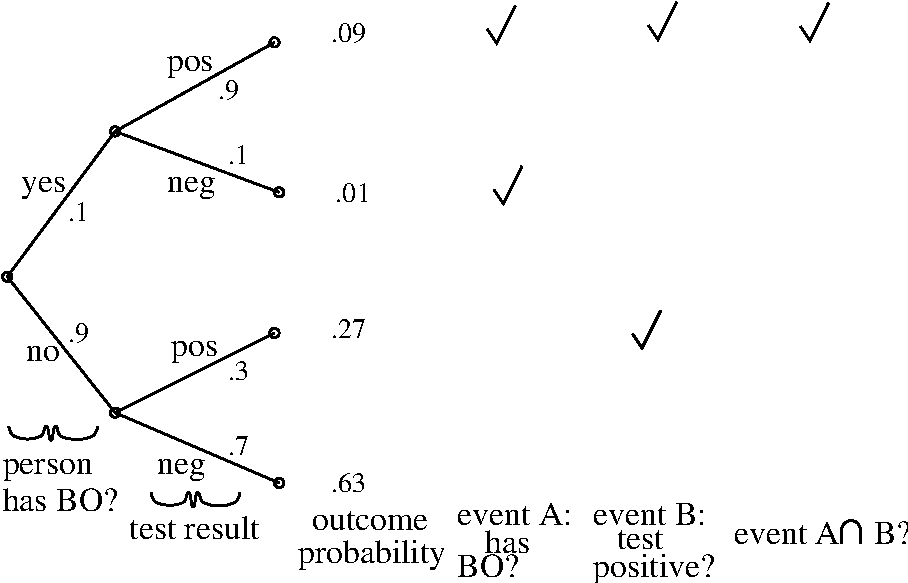
\includegraphics[height=3in]{figures/BO}
\end{center}

\subsubsection*{Step 2: Define Events of Interest}

Let $A$ be the event that the person has \emph{BO}.  Let $B$ be the
event that the test was positive.  The outcomes in each event are marked
in the tree diagram.  We want to find $\prcond{A}{B}$, the probability
that a person has \emph{BO}, given that the test was positive.

\subsubsection*{Step 3: Find Outcome Probabilities}

First, we assign probabilities to edges.  These probabilities are drawn
directly from the problem statement.  By the Product Rule, the
probability of an outcome is the product of the probabilities on the
corresponding root-to-leaf path.  All probabilities are shown in the
figure.

\subsubsection*{Step 4: Compute Event Probabilities}
p
\begin{align*}
\prcond{A}{B}	& = \frac{\pr{A \intersect B}}{\pr{B}} \\
		& = \frac{0.09}{0.09 + 0.27} \\
		& = \frac{1}{4}
\end{align*}
%
If you test positive, then there is only a 25\% chance that you have
the condition!

This answer is initially surprising, but makes sense on reflection.
There are two ways you could test positive.  First, it could be that
you are sick and the test is correct.  Second, it could be that you
are healthy and the test is incorrect.  The problem is that almost
everyone is healthy; therefore, most of the positive results arise
from incorrect tests of healthy people!

We can also compute the probability that the test is correct for a
random person.  This event consists of two outcomes.  The person could
be sick and the test positive (probability $0.09$), or the person
could be healthy and the test negative (probability $0.63$).
Therefore, the test is correct with probability $0.09 + 0.63 = 0.72$.
This is a relief; the test is correct almost three-quarters of the
time.

But wait!  There is a simple way to make the test correct 90\% of the
time: always return a negative result!  This ``test'' gives the right
answer for all healthy people and the wrong answer only for the 10\%
that actually have the condition.  The best strategy is to completely
ignore the test result!

There is a similar paradox in weather forecasting.  During winter,
almost all days in Boston are wet and overcast.  Predicting miserable
weather every day may be more accurate than really trying to get it
right!

\subsection{Conditional Identities}\label{cond_ident_subsec}

The probability rules above extend to probabilities conditioned on the
same event.  For example, the Inclusion-Exclusion formula for two sets
holds when all probabilities are conditioned on an event $C$:
\[
\prcond{A \cup B}{C} = \prcond{A}{C} + \prcond{B}{C} - \prcond{A \intersect B}{C}.
\]
This follows from the fact that if $\pr{C} \neq 0$ and we define
\[
\prsub{A}{C} \eqdef \prcond{A}{C}
\]
then $\prsub{}{C}$ satisfies the definition of being probability function.

It is important not to mix up events before and after the conditioning bar.
For example, the following is \textit{not} a valid identity:
%
\begin{falseclm*}
\begin{equation}\label{LN12:fc}
\prcond{A}{B \cup C} = \prcond{A}{B} + \prcond{A}{C} - \prcond{A}{B \intersect C}.
\end{equation}
\end{falseclm*}

A counterexample is shown below.  In this case, $\prcond{A}{B} = 1$,
$\prcond{A}{C} = 1$, and $\prcond{A}{B \cup C} = 1$.  However, since
$1 \neq 1 + 1$, the equation above does not hold.
%
\begin{center}
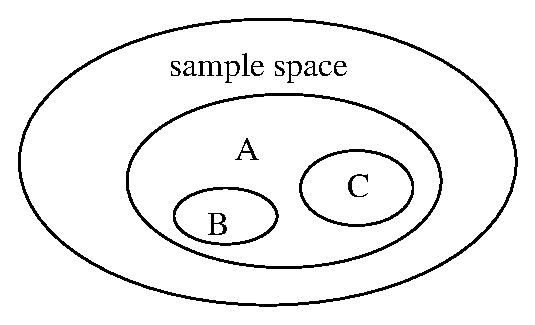
\includegraphics[height=1.5in]{figures/cx19}
\end{center}
%
So you're convinced that this equation is false in general, right?
Let's see if you \textit{really} believe that.

\subsection{Discrimination Lawsuit}\label{discrimination_subsec}

Several years ago there was a sex discrimination lawsuit against
Berkeley.  A female professor was denied tenure, allegedly because she
was a woman.  She argued that in every one of Berkeley's 22
departments, the percentage of male applicants accepted was greater
than the percentage of female applicants accepted.  This sounds very
suspicious!

However, Berkeley's lawyers argued that across the whole university
the percentage of male tenure applicants accepted was actually
\textit{lower} than the percentage of female applicants accepted.
This suggests that if there was any sex discrimination, then it was
against men!  Surely, at least one party in the dispute must be lying.

Let's simplify the problem and express both arguments in terms of
conditional probabilities.  Suppose that there are only two
departments, EE and CS, and consider the experiment where we pick a
random applicant.  Define the following events:
%
\begin{itemize}
\item Let $A$ be the event that the applicant is accepted.
\item Let $F_{EE}$ the event that the applicant is a female applying to EE.
\item Let $F_{CS}$ the event that the applicant is a female applying to CS.
\item Let $M_{EE}$ the event that the applicant is a male applying to EE.
\item Let $M_{CS}$ the event that the applicant is a male applying to
CS.
\end{itemize}
%
Assume that all applicants are either male or female, and that no
applicant applied to both departments.  That is, the events $F_{EE}$,
$F_{CS}$, $M_{EE}$, and $M_{CS}$ are all disjoint.

In these terms, the plaintiff is make the following argument:
%
\begin{align*}
\prcond{A}{F_{EE}} & < \prcond{A}{M_{EE}} \\
\prcond{A}{F_{CS}} & < \prcond{A}{M_{CS}}
\end{align*}
%
That is, in both departments, the probability that a woman is accepted
for tenure is less than the probability that a man is accepted.  The
university retorts that overall a woman applicant is \textit{more}
likely to be accepted than a man:
%
\[
\prcond{A}{F_{EE} \cup F_{CS}} > \prcond{A}{M_{EE} \cup M_{CS}}
\]

It is easy to believe that these two positions are contradictory.  In
fact, we might even try to prove this by adding the plaintiff's two
inequalities and then arguing as follows:
%
\begin{align*}
&& \prcond{A}{F_{EE}} + \prcond{A}{F_{CS}} & < 
	\prcond{A}{M_{EE}} + \prcond{A}{M_{CS}} \\
\Rightarrow && 
\prcond{A}{F_{EE} \cup F_{CS}} & <
	\prcond{A}{M_{EE} \cup M_{CS}}
\end{align*}
%
The second line exactly contradicts the university's position!  But there
is a big problem with this argument; the second inequality follows from
the first only if we accept the false identity~\eqref{LN12:fc}.  This argument
is bogus!  Maybe the two parties do not hold contradictory positions after
all!

In fact, the table below shows a set of application statistics for
which the assertions of both the plaintiff and the university hold:
%
\[
\begin{array}{crr}
\mbox{CS} & \mbox{0 females accepted, 1 applied} & 0\% \\
          & \mbox{50 males accepted, 100 applied} & 50\% \\
\mbox{EE} & \mbox{70 females accepted, 100 applied} & 70\% \\
          & \mbox{1 male accepted, 1 applied} & 100\% \\
\hline
\mbox{Overall} & \mbox{70 females accepted, 101 applied} & \approx 70\% \\
          & \mbox{51 males accepted, 101 applied} & \approx 51\%
\end{array}
\]
%
In this case, a higher percentage of males were accepted in both
departments, but overall a higher percentage of females were accepted!
Bizarre!

\subsection{\textit{A Posteriori} Probabilities}\label{aposteriori_subsec}

Suppose that we turn the hockey question around: what is the
probability that the Halting Problem won their first game, given that
they won the series?

This seems like an absurd question!  After all, if the Halting Problem
won the series, then the winner of the first game has already been
determined.  Therefore, who won the first game is a question of fact,
not a question of probability.  However, our mathematical theory of
probability contains no notion of one event preceding another--- there
is no notion of time at all.  Therefore, from a mathematical
perspective, this is a perfectly valid question.  And this is also a
meaningful question from a practical perspective.  Suppose that you're
told that the Halting Problem won the series, but not told the results
of individual games.  Then, from your perspective, it makes perfect
sense to wonder how likely it is that The Halting Problem won the
first game.

A conditional probability $\prcond{B}{A}$ is called  \term{a
posteriori} if event $B$ precedes event $A$ in time.  Here are some
other examples of a posteriori probabilities:
%
\begin{itemize}
\item The probability it was cloudy this morning, given that it rained
in the afternoon.
\item The probability that I was initially dealt two queens in Texas
No Limit Hold 'Em poker, given that I eventually got four-of-a-kind.
\end{itemize}
%
Mathematically, a posteriori probabilities are \textit{no different}
from ordinary probabilities; the distinction is only at a higher,
philosophical level.  Our only reason for drawing attention to them is
to say, ``Don't let them rattle you.''

Let's return to the original problem.  The probability that the
Halting Problem won their first game, given that they won the series
is $\prcond{B}{A}$.  We can compute this using the definition of
conditional probability and our earlier tree diagram:
%
\begin{align*}
\prcond{B}{A} & = \frac{\pr{B \intersect A}}{\pr{A}} \\
              & = \frac{1/3 + 1/18}{1/3 + 1/18 + 1/9} \\
              & = \frac{7}{9}
\end{align*}

This answer is suspicious!  In the preceding section, we showed that
$\prcond{A}{B}$ was also $7/9$.  Could it be true that $\prcond{A}{B}
= \prcond{B}{A}$ in general?  Some reflection suggests this is
unlikely.  For example, the probability that I feel uneasy, given that
I was abducted by aliens, is pretty large.  But the probability that I
was abducted by aliens, given that I feel uneasy, is rather small.

Let's work out the general conditions under which $\prcond{A}{B} =
\prcond{B}{A}$.  By the definition of conditional probability, this
equation holds if an only if:
%
\[
\frac{\pr{A \intersect B}}{\pr{B}} = \frac{\pr{A \intersect B}}{\pr{A}}
\]
%
This equation, in turn, holds only if the denominators are equal or
the numerator is 0:
%
\[
\pr{B} = \pr{A}
\hspace{0.25in} \text{or} \hspace{0.25in}
\pr{A \intersect B} = 0
\]
%
The former condition holds in the hockey example; the probability that
the Halting Problem wins the series (event $A$) is equal to the
probability that it wins the first game (event $B$).  In fact, both
probabilities are $1/2$.

%\iffalse
Such pairs of probabilities are related by \idx{Bayes' Rule}:
%
\begin{theorem}[Bayes' Rule]
If $\pr{A}$ and $\pr{B}$ are nonzero, then:
%
\begin{equation}\label{bayesrule}
\frac{\prcond{A}{B} \cdot \pr{B}}{\pr{A}} = \prcond{B}{A}
\end{equation}
\end{theorem}

\begin{proof}
When $\pr{A}$ and $\pr{B}$ are nonzero, we have
\[
\prcond{A}{B} \cdot \pr{B} = \prob{A \intersect B} = \prcond{B}{A} \cdot \pr{A}
\]
by definition of conditional probability.  Dividing by $\prob{A}$
gives~\eqref{bayesrule}.

\end{proof}

In the hockey problem, the probability that the Halting Problem wins the
first game is $1/2$ and so is the probability that the Halting Problem
wins the series.  Therefore, $\pr{A} = \pr{B} = 1/2$.  This, together with
Bayes' Rule, explains why $\prcond{A}{B}$ and $\prcond{B}{A}$ turned out to
be equal in the hockey example.

%% Conditional Probability Problems %%%%%%%%%%%%%%%%%%%%%%%%%%%%%%%%%%%%%%%%%%%

\begin{problems}
\practiceproblems
\pinput{TP_six_shooter_probability}

\classproblems
\pinput{CP_missing_card_probability}
\pinput{CP_conditional_prob_says_so_bug}

\homeworkproblems
\pinput{PS_conditional_probability_problem_errors}
\pinput{PS_coin_flip_sequences}
\pinput{PS_13_card_hand}
\pinput{PS_neighborhood_census}
\end{problems}

%% Independence %%%%%%%%%%%%%%%%%%%%%%%%%%%%%%%%%%%%%%%%%%%%%%%%%%%%%%%%%%%%%%%
\section{Independence}

Suppose that we flip two fair coins simultaneously on opposite sides
of a room.  Intuitively, the way one coin lands does not affect the
way the other coin lands.  The mathematical concept that captures
this intuition is called \term{independence}:
\begin{definition*}
Events $A$ and $B$ are independent if and only if:
\[
\pr{A \intersect B} = \pr{A} \cdot \pr{B}
\]
\end{definition*}
Generally, independence is something you \textit{assume} in modeling a
phenomenon--- or wish you could realistically assume.  Many useful
probability formulas only hold if certain events are independent, so a
dash of independence can greatly simplify the analysis of a system.

\subsection{Examples}

Let's return to the experiment of flipping two fair coins.  Let $A$ be
the event that the first coin comes up heads, and let $B$ be the event
that the second coin is heads.  If we assume that $A$ and $B$ are
independent, then the probability that both coins come up heads is:
%
\begin{align*}
\pr{A \intersect B} & = \pr{A} \cdot \pr{B} \\
              & = \frac{1}{2} \cdot \frac{1}{2} \\
              & = \frac{1}{4}
\end{align*}

On the other hand, let $C$ be the event that tomorrow is cloudy and
$R$ be the event that tomorrow is rainy.  Perhaps $\pr{C} = 1/5$ and
$\pr{R} = 1/10$ around here.  If these events were independent, then
we could conclude that the probability of a rainy, cloudy day was
quite small:
%
\begin{align*}
\pr{R \intersect C} & = \pr{R} \cdot \pr{C} \\
              & = \frac{1}{5} \cdot \frac{1}{10} \\
              & = \frac{1}{50}
\end{align*}
%
Unfortunately, these events are definitely not independent; in
particular, every rainy day is cloudy.  Thus, the probability of a
rainy, cloudy day is actually $1/10$.

\subsection{Working with Independence}

There is another way to think about independence that you may find more
intuitive.  According to the definition, events $A$ and $B$ are
independent if and only if $\pr{A \intersect B} = \pr{A} \cdot \pr{B}$.  This
equation holds even if $\pr{B} = 0$, but assuming it is not, we can divide
both sides by $\pr{B}$ and use the definition of conditional probability
to obtain an alternative formulation of independence:
\begin{proposition*}
If $\pr{B} \neq 0$, then
events $A$ and $B$  are independent if and only if
\begin{equation}\label{LN12:ABA}
\prcond{A}{B} = \pr{A}.
\end{equation}
\end{proposition*}

Equation~\eqref{LN12:ABA} says that events $A$ and $B$ are independent if the
probability of $A$ is unaffected by the fact that $B$ happens.  In these
terms, the two coin tosses of the previous section were independent,
because the probability that one coin comes up heads is unaffected by the
fact that the other came up heads.  Turning to our other example, the
probability of clouds in the sky is strongly affected by the fact that it
is raining.  So, as we noted before, these events are not independent.

\textbf{Warning:} Students sometimes get the idea that disjoint events are
independent.  The \emph{opposite} is true: if $A \intersect B =
\emptyset$, then knowing that $A$ happens means you know that $B$ does not
happen.  So disjoint events are \emph{never} independent ---unless one of
them has probability zero.

\begin{staffnotes}

\subsection{Some Intuition}

Suppose that $A$ and $B$ are disjoint events, as shown in the figure
below.
%
\begin{center}
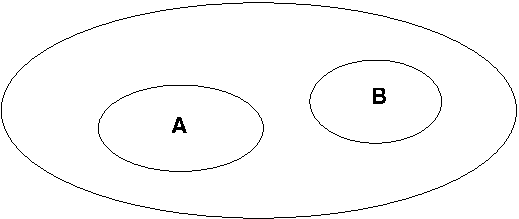
\includegraphics{figures/disjoint-events}
\end{center}
%
Are these events independent?  Let's check.  On one hand, we know
%
\[
\pr{A \intersect B} = 0
\]
%
because $A \intersect B$ contains no outcomes.  On the other hand, we have
%
\[
\pr{A} \cdot \pr{B} > 0
\]
%
except in degenerate cases where $A$ or $B$ has zero probability.
Thus, \textit{disjointness and independence are very different ideas}.

Here's a better mental picture of what independent events look like.
%
\begin{center}
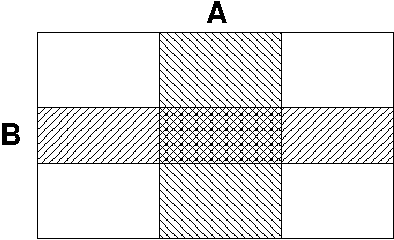
\includegraphics{figures/independent-events}
\end{center}
%
The sample space is the whole rectangle.  Event $A$ is a vertical
stripe, and event $B$ is a horizontal stripe.  Assume that the
probability of each event is proportional to its area in the diagram.
Now if $A$ covers an $\alpha$-fraction of the sample space, and $B$
covers a $\beta$-fraction, then the area of the intersection region is
$\alpha \cdot \beta$.  In terms of probability:
%
\[
\pr{A \intersect B} = \pr{A} \cdot \pr{B}
\]

\end{staffnotes}


\subsection{Mutual Independence}

We have defined what it means for two events to be independent.  But
how can we talk about independence when there are more than two
events?  For example, how can we say that the orientations of $n$
coins are all independent of one another?

Events $E_1, \ldots, E_n$ are \term{mutually independent} if and only
if \textit{for every subset} of the events, the probability of the
intersection is the product of the probabilities.  In other words, all
of the following equations must hold:
%
\begin{align*}
\pr{E_i \intersect E_j}
    & = \pr{E_i} \cdot \pr{E_j}
    & \text{for all distinct $i$, $j$} \\
\pr{E_i \intersect E_j \intersect E_k}
    & = \pr{E_i} \cdot \pr{E_j} \cdot \pr{E_k}
     & \text{for all distinct $i$, $j$, $k$} \\
\pr{E_i \intersect E_j \intersect E_k \intersect E_l}
    & = \pr{E_i} \cdot \pr{E_j} \cdot \pr{E_k} \cdot \pr{E_l}
    & \text{for all distinct $i$, $j$, $k$, $l$} \\
    & \ldots \\
\pr{E_1 \intersect \cdots \intersect E_n} & = \pr{E_1} \cdots \pr{E_n}
\end{align*}
%
As an example, if we toss 100 fair coins and let $E_i$ be the event
that the $i$th coin lands heads, then we might reasonably assume that
$E_1, \dots, E_{100}$ are mutually independent.

\begin{staffnotes}

\subsection{DNA Testing}

This is testimony from the O. J. Simpson murder trial on May 15, 1995:

\textbox{
\begin{description}

\item[MR. CLARKE:] When you make these estimations of frequency--- and
I believe you touched a little bit on a concept called independence?

\item[DR. COTTON:] Yes, I did.

\item[MR. CLARKE:] And what is that again?

\item[DR. COTTON:] It means whether or not you inherit one allele that
you have is not--- does not affect the second allele that you might
get.  That is, if you inherit a band at 5,000 base pairs, that doesn't
mean you'll automatically or with some probability inherit one at
6,000.  What you inherit from one parent is what you inherit from the
other.  \emph{(Got that? -- EAL)}

\item[MR. CLARKE:] Why is that important?

\item[DR. COTTON:] Mathematically that's important because if that
were not the case, it would be improper to multiply the frequencies
between the different genetic locations.

\item[MR. CLARKE:] How do you--- well, first of all, are these markers
independent that you've described in your testing in this case?

\end{description}
}

The jury was told that genetic markers in blood found at the crime
scene matched Simpson's.  Furthermore, the probability that the
markers would be found in a randomly-selected person was at most 1 in
170 million.  This astronomical figure was derived from statistics such
as:
%
\begin{itemize}
\item 1 person in 100 has marker $A$.
\item 1 person in 50 marker $B$.
\item 1 person in 40 has marker $C$.
\item 1 person in 5 has marker $D$.
\item 1 person in 170 has marker $E$.
\end{itemize}
%
Then these numbers were multiplied to give the probability that a
randomly-selected person would have all five markers:
%
\begin{align*}
\pr{A \intersect B \intersect C \intersect D \intersect E}
    & = \pr{A} \cdot \pr{B} \cdot \pr{C} \cdot \pr{D} \cdot \pr{E} \\
    & = \frac{1}{100} \cdot \frac{1}{50} \cdot \frac{1}{40}
                      \cdot \frac{1}{5} \cdot \frac{1}{170} \\
    & = \frac{1}{170,000,000}
\end{align*}
%
The defense pointed out that this assumes that the markers appear
mutually independently.  Furthermore, all the statistics were based on
just a few hundred blood samples.  The jury was widely mocked for
failing to ``understand'' the DNA evidence.  If you were a juror,
would \textit{you} accept the 1 in 170 million calculation?

\end{staffnotes}


\subsection{Pairwise Independence}

The definition of mutual independence seems awfully complicated---
there are so many conditions!  Here's an example that illustrates the
subtlety of independence when more than two events are involved and
the need for all those conditions.  Suppose that we flip three fair,
mutually-independent coins.  Define the following events:
%
\begin{itemize}
\item $A_1$ is the event that coin 1 matches coin 2.
\item $A_2$ is the event that coin 2 matches coin 3.
\item $A_3$ is the event that coin 3 matches coin 1.
\end{itemize}
%
Are $A_1$, $A_2$, $A_3$ mutually independent?

The sample space for this experiment is:
%
\[
\set{HHH,\ HHT,\ HTH,\ HTT,\ THH,\ THT,\ TTH,\ TTT}
\]
%
Every outcome has probability $(1/2)^3 = 1/8$ by our assumption that
the coins are mutually independent.

To see if events $A_1$, $A_2$, and $A_3$ are mutually independent, we
must check a sequence of equalities.  It will be helpful first to
compute the probability of each event $A_i$:
%
\begin{align*}
\pr{A_1} & = \pr{HHH} + \pr{HHT} + \pr{TTH} + \pr{TTT} \\
         & = \frac{1}{8} + \frac{1}{8} + \frac{1}{8} + \frac{1}{8}\\
         & = \frac{1}{2}
\end{align*}
%
By symmetry, $\pr{A_2} = \pr{A_3} = 1/2$ as well.  Now we can begin
checking all the equalities required for mutual independence.
%
\begin{align*}
\pr{A_1 \intersect A_2}
	& = \pr{HHH} + \pr{TTT} \\
        & = \frac{1}{8} + \frac{1}{8} \\
        & = \frac{1}{4} \\
        & = \frac{1}{2} \cdot \frac{1}{2}\\
        & = \pr{A_1} \pr{A_2}
\end{align*}
%
By symmetry, $\pr{A_1 \intersect A_3} = \pr{A_1} \cdot \pr{A_3}$ and
$\pr{A_2 \intersect A_3} = \pr{A_2} \cdot \pr{A_3}$ must hold also.
Finally, we must check one last condition:
%
\begin{align*}
\pr{A_1 \intersect A_2 \intersect A_3}      & = \pr{HHH} + \pr{TTT} \\
                                & = \frac{1}{8} + \frac{1}{8} \\
                                & = \frac{1}{4} \\
                                & \neq \pr{A_1} \pr{A_2} \pr{A_3} = \frac{1}{8}
\end{align*}
%
The three events $A_1$, $A_2$, and $A_3$ are not mutually independent
even though any two of them are independent!  This not-quite
mutual independence seems weird at first, but it happens.   It even generalizes:

\begin{definition}\label{kway_independent_events}
  A set $A_0,A_1,\dots$ of events is \term{$k$-way independent} iff every
  set of $k$ of these events is mutually independent.  The set is
  \term{pairwise independent} iff it is 2-way independent.
\end{definition}

So the sets $A_1,A_2,A_3$ above are pairwise independent, but not mutually
independent.  Pairwise independence is a much weaker property than mutual
independence, but it's all that's needed to justify a standard approach to
making probabilistic estimates that will come up later.

\begin{staffnotes}

For example, suppose that the prosecutors in the
O. J. Simpson trial were wrong and markers $A$, $B$, $C$, $D$, and $E$
appear only \textit{pairwise} independently.  Then the probability
that a randomly-selected person has all five markers is no more than:
%
\begin{align*}
\pr{A \intersect B \intersect C \intersect D \intersect E}
    & \leq \pr{A \intersect E} \\
    & = \pr{A} \cdot \pr{E} \\
    & = \frac{1}{100} \cdot \frac{1}{170} \\
    & = \frac{1}{17,000}
\end{align*}
%
The first line uses the fact that $A \intersect B \intersect C \intersect
D \intersect E$ is a subset of $A \intersect E$.  (We picked out the $A$
and $E$ markers because they're the rarest.)  We use pairwise independence
on the second line.  Now the probability of a random match is 1 in
17,000--- a far cry from 1 in 170 million!  And this is the strongest
conclusion we can reach assuming only pairwise independence.

\end{staffnotes}

\begin{problems}
\classproblems
\pinput{CP_three_fair_coins}
\end{problems}


%% The Birthday Principle %%%%%%%%%%%%%%%%%%%%%%%%%%%%%%%%%%%%%%%%%%%%%%%%%%%%%
\section{The Birthday Principle}\label{birthday_principle_sec}

There are 85 students in a class.  What is the probability that some
birthday is shared by two people?  Comparing 85 students to the 365
possible birthdays, you might guess the probability lies somewhere
around $1/4$ ---but you'd be wrong: the probability that there will be
two people in the class with matching birthdays is actually more than
$0.9999$.

To work this out, we'll assume that the probability that a randomly
chosen student has a given birthday is $1/d$, where $d= 365$ in this
case.  We'll also assume that a class is composed of $n$ randomly and
independently selected students, with $n=85$ in this case.  These
randomness assumptions are not really true, since more babies are born
at certain times of year, and students' class selections are typically
not independent of each other, but simplifying in this way gives us a
start on analyzing the problem.  More importantly, these assumptions
are justifiable in important computer science applications of birthday
matching.  For example, the birthday matching is a good model for
collisions between items randomly inserted into a hash table.  So we
won't worry about things like Spring procreation preferences that make
January birthdays more common, or about twins' preferences to take
classes together (or not).  \iffalse , or that fact that a student
can't be selected twice in making up a class list.  \fi

Selecting a sequence of $n$ students for a class yields a sequence of
$n$ birthdays.  Under the assumptions above, the $d^n$ possible
birthday sequences are equally likely outcomes.  Let's examine the
consequences of this probability model by focussing on the $i$th and
$j$th elements in a birthday sequence, where $1 \leq i \neq j \leq n$.
It makes for a better story if we refer to the $i$th birthday as
``Alice's'' and the $j$th as ``Bob's.''

Now since Bob's birthday is assumed to be independent of Alice's, it
follows that whichever of the $d$ birthdays Alice's happens to be, the
probability that Bob has the same birthday $1/d$.  Next, If we look at
two other birthdays ---call them ``Carol's'' and ``Don's'' ---then
whether Alice and Bob have matching birthdays has nothing to do with
whether Carol and Don have matching birthdays.  That is, the event
that Alice and Bob have matching birthdays is independent of the event
that Carol and Don have matching birthdays.  In fact, for any set of
non-overlapping couples, the events that a couple has matching
birthdays are mutually independent.

In fact, it's pretty clear that the probability that Alice and Bob
have matching birthdays remains $1/d$ whether or not Carol and
\emph{Alice} have matching birthdays.  That is, the event that Alice
and Bob match is also independent of Alice and Carol matching.  In
short, the set of all events in which a couple has macthing birthdays
is \index{pairwise independent} \emph{pairwise} independent, despite
the overlapping couples.  This will be important in
Chapter~\ref{deviation_chap} because pairwise independence will be
enough to justify some conclusions about the expected number of
matches.  However, it's obvious that these matching birthday events
are \emph{not} \idx{mutually independent}, not even 3-way independent:
if Alice and Bob match and also Alice and Carol match, then Bob and
Carol will match.

We could justify all these assertions of independence routinely using
the four step method, but it's pretty boring, and we'll skip it.

It turns out that as long as the number of students is noticeably
smaller than the number of possible birthdays, we can get a pretty
good estimate of the birthday matching probabilities by
\emph{pretending} that the matching events are mutually independent.
(An intuitive justification for this is that with only a small number
of matching pairs, it's likely that none of the pairs overlap.)  Then
the probability of \emph{no} matching birthdays would be the same as
$r$th power of the probability that a couple does \emph{not} have
matching birthdays, where $r \eqdef \binom{n}{2}$ is the number of
couples.  That is, the probability of no matching birthdays would be
\begin{equation}\label{11dbinn2}
(1-1/d)^{\binom{n}{2}}.
\end{equation}
Using the fact that $e^x >1+x$ for all $x$,\footnote{This
  approximation is obtained by truncating the Taylor series $e^{-x} =
  1 - x + x^2/2!  - x^3/3! + \cdots$.  The approximation $e^{-x}
  \approx 1 - x$ is pretty accurate when $x$ is small.} we would conclude
that the probability of no matching birthdays is at most
\begin{equation}\label{bday-approx}
e^{-\dfrac{\binom{n}{2}}{d}}.
\end{equation}

The matching birthday problem fits in here so far as a nice example
illustrating pairwise and mutual independence.  But it's actually not
hard to justify the bound~\eqref{bday-approx} without any pretence or
any explicit consideration of independence.  Namely, there are $d (d -
1) (d - 2) \cdots (d - (n - 1))$ length $n$ sequences of distinct
birthdays.  So the probability that everyone has a different birthday
is:
\begin{align*}
\lefteqn{\frac{d (d - 1) (d - 2) \cdots (d - (n - 1))}{d^n}}\\
   & = \frac{d}{d} \cdot \frac{d-1}{d} \cdot \frac{d-2}{d} \cdots \frac{d - (n - 1)}{d}\\
   & = \paren{1 - \frac{0}{d}}
             \paren{1 - \frac{1}{d}}
             \paren{1 - \frac{2}{d}}
             \cdots
             \paren{1 - \frac{n - 1}{d}}\\
   & < e^0 \cdot e^{-1/d} \cdot e^{-2/d} \cdots e^{-(n-1)/d} 
             & \text{(since $1+x < e^x$)} \\
   & = e^{-\paren{\sum_{i=1}^{n-1} i/d}}\\
   & = e^{-\paren{n(n-1)/2d}}\\
   & = \text{the bound~\eqref{bday-approx}}.
\end{align*}

For $n=85$ and $d = 365$,~\eqref{bday-approx} is less than $1/17,000$,
which means the probability of having some pair of matching birthdays
actually is more than $1- 1/17,000 > 0.9999$.  So it would be pretty
astonishing if there were no pair of students in the class with
matching birthdays.

For $d \leq n^2/2$, the probability of no match turns out to be
asymptotically equal to the upper bound~\eqref{bday-approx}.  For $d =
n^2/2$ in particular, the probability of no match is asymptotically
equal to $1/e$.  This leads to a rule of thumb which is useful in many
contexts in computer science:

\textbox{
\begin{center}
\large The \index{birthday principle} Birthday Principle
\end{center}

If there are $d$ days in a year and $\sqrt{2d}$ people in a
room, then the probability that two share a birthday is about 
$1 - 1/e \approx 0.632$.
}

For example, the Birthday Principle says that if you have $\sqrt{2
  \cdot 365} \approx 27$ people in a room, then the probability that
two share a birthday is about $0.632$.  The actual probability is
about $0.626$, so the approximation is quite good.  

Among other applications, the Birthday Principle famously comes into
play as the basis of ``birthday attacks'' that crack certain
cryptographic systems.

\iffalse
 For example, the Principle tells how many items can be
inserted into a hash table before collisions start to happen.  \fi

\iffalse that cryptographic systems and digital signature schemes must be
hardened against.  \fi


\endinput
